\chapter{Literature}\label{chapter:literature}
There is several concepts that must be understood before beginning the take-off modeling. Additionally, CS25 can be ambiguous at best so it is important to include a discussion about the CS25 requirements as well. This section summarises the relevant take-off performance literature by describing the balanced field length (BFL) concept in \autoref{sec:BFL}. Afterwards, the relevant CS25 definitions and concepts are given, and the way the author interpreted these.

\section{Balanced Field Length}\label{sec:BFL}
BFL is one of the most important performance metric of any aircraft since it determines at what airports the aircraft is allowed to operate. The BFL is a combination of the continued take-off distance and rejected take-off distance, both in case of an engine failure. The velocity at which the engine failure occurs determines the continued and rejected take-off length.
\textbf{continued take-off distance} is the distance covered when engine failure occurs, and the pilot decides to continue the take-off with $n-1$ engines.
\textbf{rejected take-off distance} is the distance covered when engine failure occurs, and the pilot decides to reject the take-off and break.
BFL is where the continued and rejected take-off distances meet. BFL is therefore the minimum required take-off distance. An example of the BFL is given in \autoref{fig:schematic_takeoff}, as taken from Torenbeek's first book on aircraft design.

\section{CS25 Definitions}\label{sec:CS25}
It is paramount to have a firm understanding of the constraints and requirements set by legislators in CS25. Therefore, this section aims to clarify the important constraints and variables set by CS25 for take-off. The following website was consulted for speed definitions: \url{https://www.ecfr.gov/current/title-14/chapter-I/subchapter-A/part-1/section-1.2}. Some velocity definitions are elaborated on below. The others must be experimentally determined, or chosen. Afterwards, the take-off path definitions are defined and explained.

\begin{table}[!ht]
    \centering
    \resizebox{\textwidth}{!}{\begin{tabular}{cccc} \hline \hline
        \textbf{Variable}           & \textbf{Symbol} & \textbf{Definition}                                             & \textbf{Page(s) in CS25}  \\ \hline
         Reference Stall Speed      & $V_{SR}$        & Stall Speed in straight unaccelerated flight.                   & 105-107                   \\
         Critical Engine Failure    & $V_{EF}$        & Velocity at which crit. engine fails, smaller than $V_1$ -- Torenbeek states 2 seconds before $V_1$        & 105-107                   \\
         Decision speed             & $V_1$           & The speed beyond which takeoff should no longer be aborted.     & 107                       \\
         Minimum take-off speed     & $V_{2,min}$     & Minimum take-off speed.                                         & 107                       \\
         Take-off speed             & $V_{2}$         & Take-off speed, steady climb with one engine inoperative.       & 108                       \\
         Minimum unstick speed      & $V_{MU}$        & Minimum unstick speed.                                          & 108                       \\
         Minimum control speed      & $V_{MC}$        & Minimum control speed with one engine inoperative.              & 154                       \\
         Rotation speed             & $V_{R}$         & Rotation speed.                                                 & 108                       \\
         Lift-off speed             & $V_{LOF}$       & Aircraft first airborne.                                        & 108                       \\
         Final take-off speed       & $V_{LOF}$       & Must be larger than 1.18$V_{SR}$.                               & 109                       \\ \hline
    \end{tabular}}
    \caption{CS25 definitions}
    \label{tab:my_label}
\end{table}

\subsection{Stall Speed, $V_{SR}$}
According to AMC 25.103(b) on page 106 of CS25:
\begin{center}
    \textit{The airplane should be trimmed for hands-off flight at a speed 13 percent to 30 percent above the anticipated $V_{SR}$ with the engines at idle and the airplane in the configuration for which the stall speed is being determined. Then, using only the primary longitudinal control for speed reduction, a constant deceleration (entry rate) is maintained until the airplane is stalled.}
\end{center}
Please note that other stall speeds, such as in landing configuration, have different denotations. Luckily CS25 does not specify these any further so have fun determining those when you need them. Luckily there are some people who do take the effort to decently explain this speed\footnote{\url{https://code7700.com/v-sr.htm}}. In a nutshell, the \textbf{reference} stall speed is:
\begin{center}
    \textit{You should note that VSR is measured during test conditions on a fully trimmed aircraft, 1-G flight, using a measured deceleration. If you are turning, decelerating more than 1 knot per second, or have any other conditions outside what the pilots used to produce these numbers, you aircraft is going to stall at a higher speed.}
\end{center}
This means that the reference stall speed is the lowest stall speed that can be obtained. For LTO this means that this is tested at ISA=0. Perhaps this also means that your landing gear should be deployed but I couldn't find a definitive answer for this. So for now, it's just means that the reference stall speed is calculated like any other stall speed: using the $C_{L,max}$. 

\subsection{Critical Engine Failure Speed, $V_{EF}$}
Critical engine: if this engine fails, we get the largest around the zenith-axis, because engines all rotate in the same direction, and at an angle the left and right side induce a different force, thus one engine will create a larger moment.

\subsection{Take-off speed, $V_2$}
According to CS 25.107 on page 108 of CS25:
\begin{center}
    \textit{1·08 VSR for Turbo-propeller powered aeroplanes with more than three engines}
\end{center}

\subsection{Rotation speed, $V_{MC}$}
There's multiple $V_{MC}$ values, either for Air or Ground, denoted by their first letters, and whether zero, one or two engines are inoperative.

\subsection{Rotation speed, $V_R$}
According to CS 25.107 on page 108 of CS25;
\begin{center}
    \textit{Must be more than 1.05$V_{MC}$ and larger than $V_1$}
\end{center}
and;
\begin{center}
    \textit{If the aircraft is rotated at its maximum speed, the $V_{LOF}$ is still larger than 1.1$V_{MU}$ for all engines operative, and 1.05$V_{MU}$}
\end{center}

\subsection{TORA, ASDA and TODA}
The definitions TORA, ASDA and TODA are often mentioned and carry importance in take-off modeling since it determines the distance available for potential emergency manoeuvres. \autoref{fig:TORA_ASDA_TODA} details these distances and should be self-explanatory. What exact distance is relevant depends on the airport itself, since not all are always available.

\begin{figure}
    \centering
    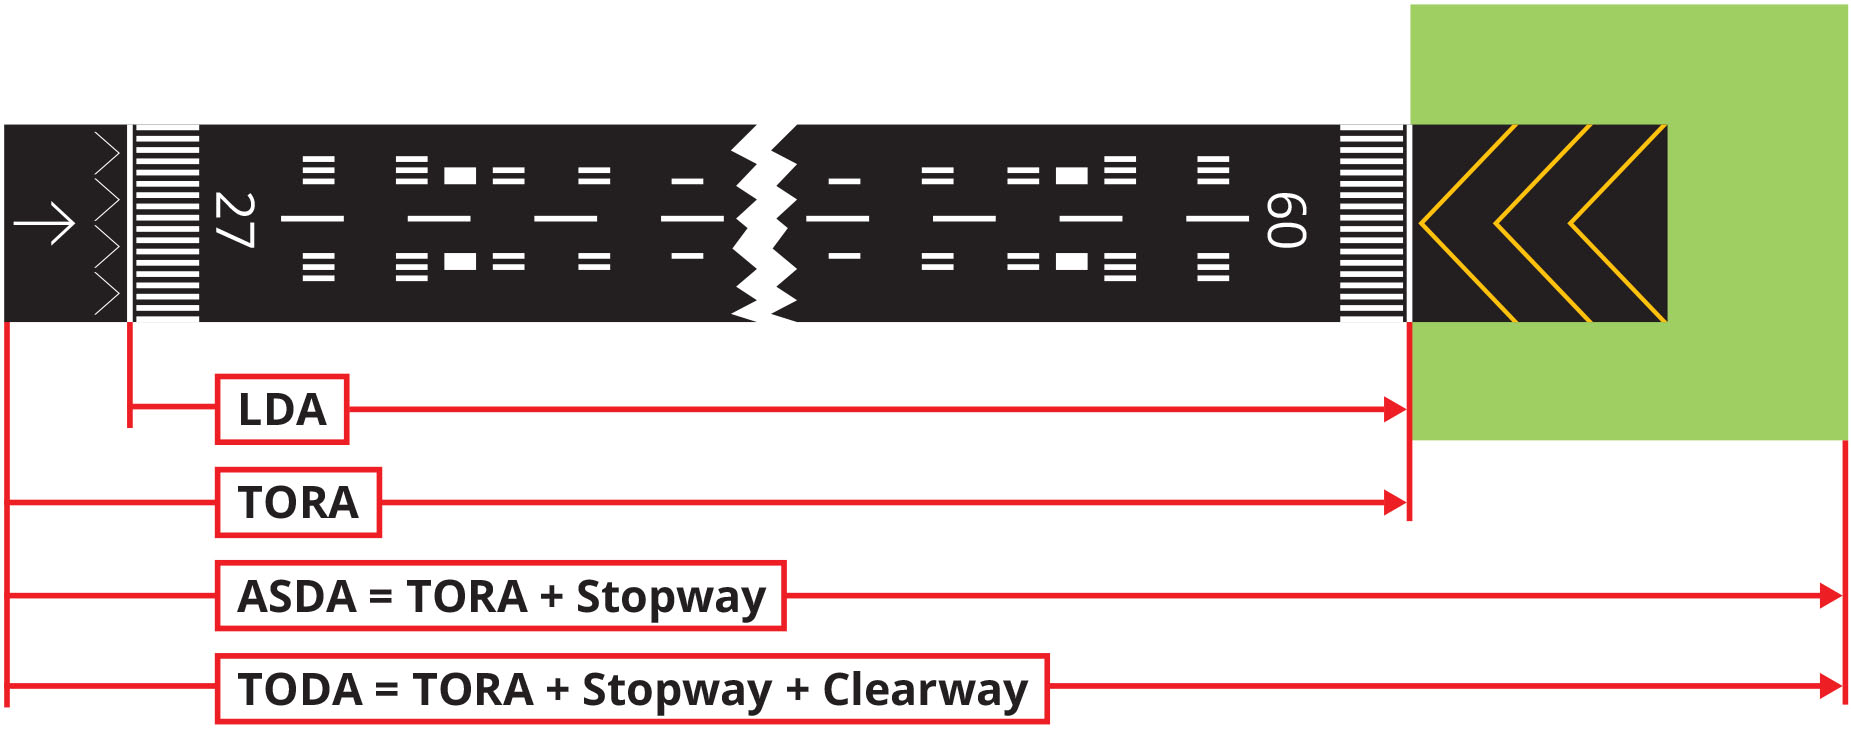
\includegraphics[width=0.75\linewidth]{figures/TORA_ASDA_TODA.jpg}
    \caption{TORA, ASDA and TODA}
    \label{fig:TORA_ASDA_TODA}
\end{figure}

\subsection{Take-off Distance and Take-Off Run}
Take-off distance is the greater of the horizontal distance from start of take-off until the aircraft has reached a screen height of 35 ft (or 11 m) with an engine failure at $V_{EF}$, or 115\% of the take-off distance with all engines operative, with the take-off distance being from standstill to the point in the middle of $V_{lof}$ and $V_2$. Additionally, if the take-off distance does not include a clearway, the take-off run is equal to the take-off distance.

\subsection{Velocity Assumptions}
To model the take-off performance, several assumptions have been made about these velocities. \autoref{tab:simulation_velocities} details what assumptions have been made about these velocities for the F9X, and thus are inputs for the models as well. Velocities that aren't mentioned in this table can therefore be assumed irrelevant for the models and should be determined afterwards. Important for all models is that the calculations go in opposite direction of what one might expect. We calculate the stall speed, from which $V_2$ follows. The model then calculates $V_r$, after which we can calculate $V_1$ and $V_{EF}$ to satisfy start-stop requirements. All of this should be done for one engine inoperative.

\begin{table}[!ht]
    \centering
    \begin{tabular}{ccc} \hline \hline
        \textbf{Variable}           & \textbf{Symbol} & \textbf{Assumption}                                             \\ \hline
         Reference Stall Speed      & $V_{SR}$        & $V_{SR} = \sqrt{\frac{2L}{\rho C_{L,max}S}}$                   \\
         Engine failure speed       & $V_{EF}$        & Calculate in model                                           \\
         Decision speed             & $V_{1}$         & Calculate in model                                           \\
         Rotation speed             & $V_{R}$         & $V_{R} \geq V_{SR}$ (calculated)                                 \\
         Final take-off speed       & $V_{LOF}$       & Must be larger than 1.0$V_{SR}$.                               \\
         Take-off speed             & $V_{2}$         & $V_{2,min}=1.08 V_{SR}$                                           \\ \hline
    \end{tabular}
    \caption{Assumptions about take-off velocities}
    \label{tab:simulation_velocities}
\end{table}

\subsection{CS25 Exceptions and Ambiguities}
The E9X is a novel aircraft, in the sense that it is electrically driven and has eight propulsors. Having eight propulsors inherently introduces the possibility of cascading failure -- where a single propeller fails and causes one/multiple of the adjacent propellers to have too. As of now, CS25 does not specify this requirement, but it could be that in the future this requirement is negotiated.

\subsection{Conclusion}
The following constraints will be implemented...